\documentclass[border=6pt]{standalone}
\usepackage{tikz}
\usetikzlibrary{arrows.meta,positioning,shapes.geometric,shapes.multipart,calc,fit,backgrounds,decorations.pathreplacing,decorations.markings,automata,chains,matrix,patterns}
\usepackage{circuitikz}
\usepackage{amsmath}
\usepackage{amssymb}
\begin{document}
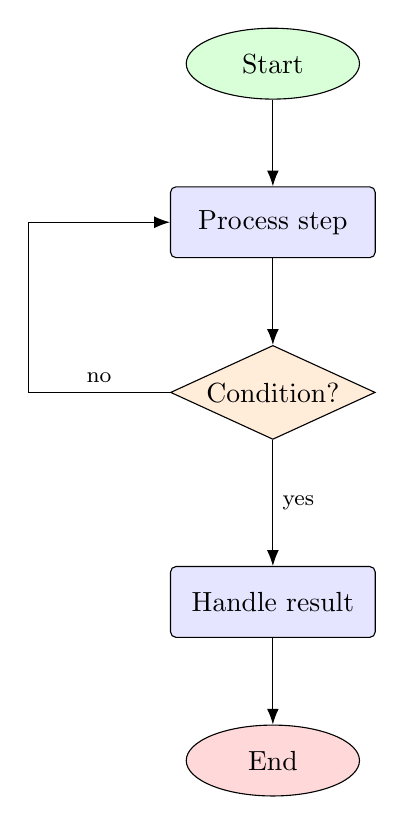
\begin{tikzpicture}[
  node distance=1.1cm,
  start/.style={ellipse, draw, fill=green!15, minimum width=2.2cm, minimum height=0.9cm},
  proc/.style={rectangle, draw, fill=blue!10, minimum width=2.6cm, minimum height=0.9cm, rounded corners=2pt},
  decision/.style={diamond, draw, fill=orange!15, aspect=2, minimum width=2.6cm, inner sep=1pt},
  arr/.style={-{Latex[length=2mm]}}
]
  \node[start] (start) {Start};
  \node[proc, below=of start] (step1) {Process step};
  \node[decision, below=of step1] (dec) {Condition?};
  \node[proc, below=1.6cm of dec] (step2) {Handle result};
  \node[start, below=of step2, fill=red!15] (end) {End};

  \draw[arr] (start) -- (step1);
  \draw[arr] (step1) -- (dec);
  \draw[arr] (dec) -- node[right, font=\footnotesize] {yes} (step2);
  \draw[arr] (step2) -- (end);
  \draw[arr] (dec.west) -- ++(-1.8,0) node[midway, above, font=\footnotesize] {no} |- (step1.west);
\end{tikzpicture}
\end{document}
